\documentclass[11pt]{article}
\usepackage[margin=1.1in]{geometry}
\usepackage{amsmath, amssymb}
\usepackage{tikz}
\usetikzlibrary{decorations.pathmorphing, arrows.meta, calc, patterns}
\usepackage[font=small, labelfont=bf]{caption}
\usepackage{url}
\setlength{\parskip}{4pt}

\title{Fried's identity at a crossing metric: the intuitive view\\
\large How a resonance walks to zero, drawn}
\author{Benjamin Lawton}
\date{September 2026 --- figures companion to the Lean statement
\texttt{fried\_counterexample\_of\_resolvent\_inputs}\\[2pt]
\small a conditional reduction from cited inputs; not yet verified by a mathematician other than the author}

\begin{document}
\maketitle

\begin{abstract}
\noindent Fried's conjecture identifies a dynamical number (the Ruelle zeta function at $s=0$)
with a topological one (Reidemeister torsion). This document draws a construction in which the
identity, as usually stated, fails: a closed hyperbolic 3-manifold with $b_1 = 1$, a unitary
character $\chi_\theta$ close to trivial, and a conformal deformation of the hyperbolic metric.
Two dials are turned. The first ($\theta$) plants a real resonance a distance $\Theta(\theta^2)$
from zero; the second (the metric) walks it to zero. At the crossing, a pole and a zero of
$\zeta$ arrive together but at different speeds, and the value $\zeta(0)$ jumps by a factor
$\Theta(\theta^2)$. Chaubet--Dang's refined identity absorbs the jump; the naive identity does
not. What is machine-checked is the reduction: granting six groups of facts cited from the
literature about the two resonance clusters near $0$, the value at the crossing is
$\tau_R \cdot (\text{pole rate})/(\text{zero rate}) \neq \tau_R$. That the geodesic flow has
those properties is taken from the cited papers and has not been verified by a mathematician
other than the author.
\end{abstract}

\section{What Fried says, and the two torsions}

Let $Z$ be a closed negatively curved manifold, $\mathcal{S} = S^*Z$ its unit cotangent bundle,
$X$ the geodesic vector field, and $\rho$ a unitary representation of $\pi_1(Z)$. The Ruelle
zeta function is a product over primitive closed geodesics $\gamma$,
\[
\zeta_{X,\rho}(s) \;=\; \prod_{\gamma} \det\!\big(1 - \varepsilon_\gamma\, \rho(\gamma)\, e^{-s\ell(\gamma)}\big),
\qquad \varepsilon_\gamma = \operatorname{sign}\det(1 - P_\gamma),
\]
so that $\log \zeta$ is a sum of Wilson loops $\operatorname{tr}\rho(\gamma^j)$ weighted by
$e^{-sj\ell(\gamma)}$. It continues meromorphically to $\mathbb{C}$; its zeros and poles are the
Pollicott--Ruelle resonances of $L_X$ acting on $E$-valued forms, counted with the sign
$(-1)^k$ of the form degree. On the topological side, if $\rho$ is acyclic ($H^\bullet(Z;\rho)=0$)
the Reidemeister torsion $\tau_R(\rho)$ is a combinatorial invariant of a triangulation, equal by
Cheeger--M\"uller to the analytic (Ray--Singer) torsion. Fried's conjecture, in the form stated
by Dang--Guillarmou--Rivi\`ere--Shen (DGRS) for acyclic unitary $\rho$, is the naive identity
\[
|\zeta_{X,\rho}(0)|^{(-1)^q} \;=\; \tau_R(\rho), \qquad q = \dim E_s ,
\]
proved by Fried for hyperbolic metrics and by DGRS for small perturbations of them. Here $q = 2$,
so the exponent is $+1$.

\begin{figure}[h]
\centering
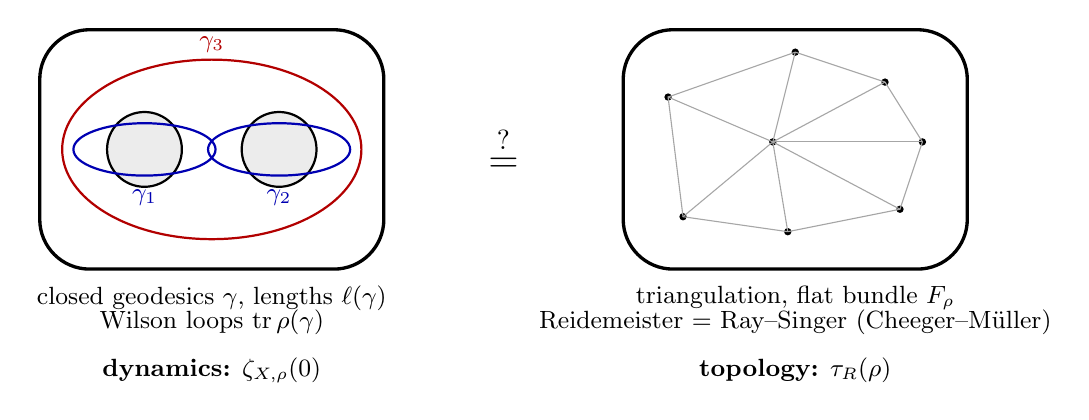
\begin{tikzpicture}[scale=0.95]
% left: manifold with closed geodesics
\begin{scope}[xshift=0cm]
\draw[very thick, rounded corners=18pt] (0,0) rectangle (4.6,3.2);
\draw[thick, fill=gray!15] (1.4,1.6) circle (0.5);
\draw[thick, fill=gray!15] (3.2,1.6) circle (0.5);
\draw[thick, blue!70!black] (1.4,1.6) ellipse (0.95 and 0.35);
\draw[thick, blue!70!black] (3.2,1.6) ellipse (0.95 and 0.35);
\draw[thick, red!70!black] (2.3,1.6) ellipse (2.0 and 1.2);
\node[blue!70!black] at (1.4,0.95) {\small $\gamma_1$};
\node[blue!70!black] at (3.2,0.95) {\small $\gamma_2$};
\node[red!70!black] at (2.3,3.0) {\small $\gamma_3$};
\node[align=center] at (2.3,-0.55) {\small closed geodesics $\gamma$, lengths $\ell(\gamma)$\\[-3pt]
\small Wilson loops $\operatorname{tr}\rho(\gamma)$};
\node[align=center] at (2.3,-1.35) {\small \textbf{dynamics:} $\zeta_{X,\rho}(0)$};
\end{scope}
% middle: equals with question mark
\node at (6.2,1.6) {\Large $\overset{?}{=}$};
% right: triangulation
\begin{scope}[xshift=7.8cm]
\draw[very thick, rounded corners=18pt] (0,0) rectangle (4.6,3.2);
\foreach \p/\q in {0.8/0.7, 2.2/0.5, 3.7/0.8, 0.6/2.3, 2.0/1.7, 3.5/2.5, 2.3/2.9, 4.0/1.7} {
  \fill (\p,\q) circle (1.4pt);
}
\draw[gray!70] (0.8,0.7) -- (2.2,0.5) -- (3.7,0.8) -- (4.0,1.7) -- (3.5,2.5) -- (2.3,2.9) -- (0.6,2.3) -- cycle;
\draw[gray!70] (0.8,0.7) -- (2.0,1.7) -- (2.2,0.5);
\draw[gray!70] (2.0,1.7) -- (3.7,0.8);
\draw[gray!70] (2.0,1.7) -- (4.0,1.7);
\draw[gray!70] (2.0,1.7) -- (3.5,2.5);
\draw[gray!70] (2.0,1.7) -- (2.3,2.9);
\draw[gray!70] (2.0,1.7) -- (0.6,2.3);
\node[align=center] at (2.3,-0.55) {\small triangulation, flat bundle $F_\rho$\\[-3pt]
\small Reidemeister $=$ Ray--Singer (Cheeger--M\"uller)};
\node[align=center] at (2.3,-1.35) {\small \textbf{topology:} $\tau_R(\rho)$};
\end{scope}
\end{tikzpicture}
\caption{The identity to test. Left: the dynamical side counts closed geodesics, each weighted by
the trace of its holonomy. Right: the topological side is a combinatorial determinant, which by
Cheeger--M\"uller equals a spectral determinant of Laplacians. Fried asks whether the two agree at
$s = 0$. On the metrics drawn in \S5--\S7 they do not.}
\end{figure}

\noindent The plan is to keep $\rho$ acyclic (so $\tau_R$ is defined and $\zeta(0)$ is finite
and nonzero at the hyperbolic metric) and to move the metric until a resonance of $L_X$ sits
exactly at $s = 0$. The order of $\zeta$ there is $\sum_k (-1)^k c_k$, where $c_k$ is the number
of degree-$k$ resonant states at $0$; the value of $\zeta(0)$ is a separate question, and it is
the value that fails.

\paragraph{Vocabulary shared with the Lean statement.} Near $s = 0$ the resonances of interest
form two small clusters: a rank-2 cluster in degree 1, encoded by a $2\times 2$ matrix
$M(\theta,\tau)$, and a rank-4 cluster in degree 2, encoded by a $4\times 4$ matrix
$A(\theta,\tau)$. A \emph{branch} is one eigenvalue of a cluster matrix followed continuously in
$(\theta,\tau)$. Degree 1 has the \emph{closed branch} and the \emph{twin}. Degree 2 has the two
\emph{locked branches} (the eigenvalues of $M$, lifted by $d_0$) and two \emph{pure branches}, the
roots of $Q = X^2 - e_1 X + e_2$; the pure branch nearest $0$ is written $z$. The six figures
of \S3--\S7 are these four branches; \S2 is the argument without pictures.

\section{The argument in one page}

\paragraph{Signs and counts.} For the geodesic flow of a 3-manifold ($q = \dim E_s = 2$) a
resonance of $L_X$ on $k$-forms is a zero of $\zeta$ when $k$ is even and a pole when $k$ is odd.
Write $c_k(\lambda_0)$ for the algebraic multiplicity of $\lambda_0$ as a degree-$k$ resonance:
the dimension of the generalized eigenspace, equivalently the rank of the Riesz projector for a
small disc around $\lambda_0$ in degree $k$. It is unsigned, and a Jordan block counts by its
size. The order of $\zeta$ at $\lambda_0$ is the alternating sum
\[
\operatorname{ord}_{\lambda_0}\zeta \;=\; \sum_k (-1)^k c_k(\lambda_0)
\;=\; (\text{zeros at }\lambda_0) - (\text{poles at }\lambda_0),
\]
positive for a zero, negative for a pole, $0$ for a regular nonvanishing point.

\paragraph{At the hyperbolic metric.} For the character $\chi_\theta$, $\theta \neq 0$ small,
the twisted Laplacian on functions has a bottom eigenvalue $\mu_0(\theta) = \Theta(\theta^2)$,
and the Dyatlov--Faure--Guillarmou correspondence turns it into a real scalar resonance
\[
s^*(\theta) \;=\; -1 + \sqrt{1 - \mu_0(\theta)} \;\approx\; -\tfrac{1}{2}\mu_0(\theta) \;<\; 0,
\qquad s^*(\theta) \to 0 \text{ as } \theta \to 0
\]
(\S3): the \emph{double point}, the place where everything below starts. The cluster at
$s^*(\theta)$ is $c = (1,2,3,2,1)$ (\S4): one scalar state $f$; two degree-1 states, namely $d_0 f$, the lift of $f$, which is
the \emph{closed branch} (locked to the scalar resonance, it goes wherever $f$ goes), and
$I\,d_0 f$, its rotation by a quarter turn in $E_u \oplus E_s$, which is the \emph{twin} (it
exists only because the hyperbolic metric is conformal on $E_u$, and is tied to nothing); and
their lifts and duals. Its order is $1-2+3-2+1 = +1$, Fried's simple zero. Each of the two
degree-1 states is a pole on its own; the zero is the net of the whole cluster. The degree-1
cluster has rank two, which is why the Lean statement encodes it by a $2\times 2$ matrix $M$.

\paragraph{Turning $\tau$.} The conformal deformation splits the double point. The scalar
resonance $s^*$ drifts only at rate $O(\theta^2)$ and never reaches $0$: a degree-0 resonant state
at $0$ would be a flow-invariant twisted function, a class in $H^0(Z;\chi_\theta) = 0$, so
$c_0 = 0$ at every metric of the family (DGRS Lemma 7.4). The closed branch, locked to it, stays
near $s^*$ as well. The twin leaves at rate $r_0 > 0$, dragging its lifts with it:
$d_0 u_{\mathrm{nc}}$ in degree 2 (a zero) and $d\alpha\wedge u_{\mathrm{nc}}$ in degree 3 (a
pole), locked to it because $d_0$ commutes with the flow. The travelling chain is
$(0,1,1,1,0)$, of order $-1+1-1 = -1$: a simple pole. Its position $s_{\mathrm{nc}}(\theta,\tau)$
is real (the resonance set is symmetric under $s \mapsto \bar s$) and increases from
$s^*(\theta) < 0$, so by the intermediate value theorem it vanishes at a unique
$\tau = \sigma(\theta)$. At $g_{\sigma}$ the number $0$ is a genuine degree-1 resonance.

\paragraph{Exactness forces order $0$, not $+1$.} At the crossing, acyclicity gives
$c_0 = c_4 = 0$ (DGRS Lemma 7.4), Hodge duality gives $c_3 = c_1$, and exactness of the reduced
complex $C^1_0 \to C^2_0 \to C^3_0$ (Dang--Rivi\`ere) gives $c_2 = c_1 + c_3 = 2c_1$: the middle
space is the image of the first map plus what maps onto the third. So
$\sum_k (-1)^k c_k = -c_1 + 2c_1 - c_1 = 0$ whenever the complex at $0$ is exact. Order $+1$ is
what happens at $s^*$ at $g_{\mathrm{hyp}}$, where the degree-0 state $f$ is also present; at the
crossing there is no degree-0 state at $0$, so the order is $0$: $\zeta(\cdot\,; g_\sigma)$ is
holomorphic and nonvanishing at $\lambda = 0$, and $\zeta(0; g_\sigma)$ is an ordinary value of
the meromorphic continuation, exactly as in Fried's identity itself.

\paragraph{Who supplies the second degree-2 state.} The twin is the only degree-1 state at $0$,
so $c_1 = 1$ and exactness demands $c_2 = 2$. Degree 2 near $0$ holds four branches (the
$4\times 4$ matrix $A$): the lift of the closed branch, which sits near $s^* \neq 0$ and is
unavailable; the lift of the twin, which supplies one; and the two \emph{pure} roots of
$Q = X^2 - e_1 X + e_2$. The second state at $0$ must therefore be a pure root, so
$e_2(\theta,\sigma) = 0$; and since the multiplicity is exactly $2$, only one pure root is at
$0$, so $e_1(\theta,\sigma) \neq 0$. Call the arriving pure root $z$. Its partner, the spectator,
sits at $e_1(\theta,\sigma)$, off $0$ because $\theta \neq 0$ (at $\theta = 0$ both pure roots
are pinned at $0$ for every $\tau$). Nothing ties $z$ to the twin along the way: they coincide at
the endpoint because exactness demands it, and nowhere else.

\paragraph{The value.} Near the crossing Chaubet--Dang's factorisation, read at $\lambda = 0$,
gives $\zeta(\lambda; g_\tau) = F(\lambda,\tau)\,(\lambda - z(\tau))/(\lambda - s_{\mathrm{nc}}(\tau))$
with $F$ holomorphic, nonvanishing and continuous in $\tau$: the finite cluster factor split off
from the rest of the resolvent. At $\tau = \sigma$ the factor is $\lambda/\lambda = 1$, so
$\zeta(0; g_\sigma) = F(0,\sigma)$. Off the crossing $\zeta(0; g_\tau) = \tau_R$ (DGRS Thm~2 plus
Fried at $g_{\mathrm{hyp}}$), hence $F(0,\tau) = \tau_R\, s_{\mathrm{nc}}(\tau)/z(\tau)$. Both
branches cross $0$ linearly in $\tau$, so continuity of $F$ gives
\[
\zeta(0; g_\sigma) \;=\; \tau_R \cdot \frac{s_{\mathrm{nc}}'(\sigma)}{z'(\sigma)}
\;=\; \tau_R \cdot \frac{\text{pole rate}}{\text{zero rate}} .
\]
The only limit in the argument is this one, and it is a limit of the continuous factor $F$.
The pole's rate is $r_0$ up to small corrections. The zero's rate is $\partial_\tau e_2 / e_1$,
because the two pure roots multiply to $e_2$ and the spectator is parked at $e_1$: the closer the
spectator sits to $0$, the steeper $z$ must arrive. The Lean statement certifies that the twin's
rate is at most $2r_0$ and the zero's slope exceeds $2r_0$ in modulus, so the ratio is not $1$;
informally it is $\Theta(\theta^2)$. Fried's identity would need the two speeds to be equal.

\paragraph{What survives.} The ratio is the torsion of the zero cluster (Lemma~A), so
Chaubet--Dang's refined identity, cluster torsion included, holds at the crossing; the naive
identity of \S1 does not. Sections \S3--\S7 draw each step.

\section{The dial $\theta$: a character near trivial makes a small eigenvalue}

Take $Z$ a closed hyperbolic 3-manifold with $b_1(Z) = 1$, $\omega$ the harmonic 1-form
generating $H^1$, and the family of unitary characters
$\chi_\theta = \exp\!\big(i\theta\!\int\!\omega\big)$. For small $\theta \neq 0$ the character is
acyclic (the Alexander polynomial has finitely many roots on the unit circle), so $\tau_R(\chi_\theta)$
is defined. The price of being near trivial is a small eigenvalue: the twisted Laplacian on
functions has $\Delta_\theta = \Delta + \theta A + \theta^2|\omega|^2$ with $A\cdot 1 = 0$, so its
bottom eigenvalue is
\[
\mu_0(\theta) \;=\; \theta^2\,\frac{\|\omega\|^2_{L^2}}{\operatorname{vol}(Z)} + O(\theta^4),
\qquad \mu_0(\theta) \to 0 \text{ as } \theta \to 0 .
\]
The Dyatlov--Faure--Guillarmou correspondence turns Laplace eigenvalues into scalar
(degree-0) resonances: with the convention $(L_X + s)u = 0$, each $\mu_j$ produces the pair
$s = -1 \pm \sqrt{1 - \mu_j}$. For $\mu_0$ both roots are real and simple:
\[
s^*(\theta) = -1 + \sqrt{1-\mu_0} = -\tfrac{\mu_0}{2} - \tfrac{\mu_0^2}{8} - \cdots \;\approx\; -\tfrac{\mu_0(\theta)}{2},
\qquad -1 - \sqrt{1-\mu_0} \;\approx\; -2 + \tfrac{\mu_0}{2}.
\]
As $\theta \to 0$ the first slides toward $0$ and the second toward $-2$. Everything else in the
spectrum near the real axis stays a fixed distance away: the trace-free sector lives on the band
$\operatorname{Re} s = -1$ (a Bochner margin), and the coclosed 1-form sector sits at $\pm i\sqrt{\mu_1}$
with $\mu_1$ bounded below uniformly in $\theta$, because the one small eigenform of the twisted
Hodge Laplacian on 1-forms is exact and cancels against functions. In the Lean statement this is
the hypothesis \texttt{hdouble}: $s^*(0) = 0$, $s^*$ continuous at $0$, $s^*(\theta) < 0$ for
$\theta \neq 0$.

\begin{figure}[h]
\centering
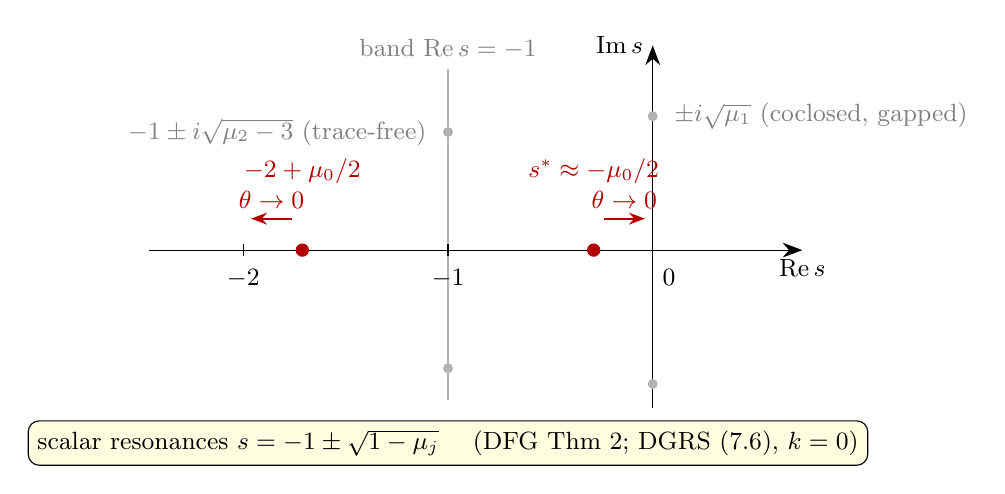
\begin{tikzpicture}[scale=1.0]
% axes
\draw[-{Stealth[length=2.5mm]}] (-6.4,0) -- (1.9,0) node[below] {\small $\operatorname{Re} s$};
\draw[-{Stealth[length=2.5mm]}] (0,-2.0) -- (0,2.6) node[left] {\small $\operatorname{Im} s$};
% band Re s = -1
\draw[thick, gray!60] (-2.6,-1.9) -- (-2.6,2.3);
\node[gray, align=center, anchor=south] at (-2.6,2.3) {\small band $\operatorname{Re} s = -1$};
\fill[gray!60] (-2.6,1.5) circle (1.8pt);
\fill[gray!60] (-2.6,-1.5) circle (1.8pt);
\node[gray, anchor=east] at (-2.75,1.5) {\small $-1 \pm i\sqrt{\mu_2 - 3}$ (trace-free)};
% coclosed sector on imaginary axis
\fill[gray!60] (0,1.7) circle (1.8pt);
\fill[gray!60] (0,-1.7) circle (1.8pt);
\node[gray, anchor=west] at (0.15,1.7) {\small $\pm i\sqrt{\mu_1}$ (coclosed, gapped)};
% ticks
\draw (-5.2,-0.08) -- (-5.2,0.08); \node[below] at (-5.2,-0.12) {\small $-2$};
\draw (-2.6,-0.08) -- (-2.6,0.08); \node[below] at (-2.6,-0.12) {\small $-1$};
\node[below right] at (0,-0.12) {\small $0$};
% the two real scalar resonances: dots on the axis, arrows above, names above the arrows
\fill[red!70!black] (-0.75,0) circle (2.4pt);
\draw[-{Stealth[length=2mm]}, thick, red!70!black] (-0.62,0.4) -- (-0.1,0.4)
  node[midway, above, red!70!black] {\small $\theta \to 0$};
\node[red!70!black] at (-0.75,1.0) {\small $s^* \approx -\mu_0/2$};
\fill[red!70!black] (-4.45,0) circle (2.4pt);
\draw[-{Stealth[length=2mm]}, thick, red!70!black] (-4.58,0.4) -- (-5.1,0.4)
  node[midway, above, red!70!black] {\small $\theta \to 0$};
\node[red!70!black] at (-4.45,1.0) {\small $-2 + \mu_0/2$};
% formula box
\node[draw, rounded corners, fill=yellow!12, align=center] at (-2.6,-2.45)
  {\small scalar resonances $s = -1 \pm \sqrt{1-\mu_j}$ \quad (DFG Thm 2; DGRS (7.6), $k=0$)};
\end{tikzpicture}
\caption{The first dial. In the $s$-plane, the small twisted eigenvalue $\mu_0(\theta)$ produces
two simple \emph{real} scalar resonances; the one at $s^*(\theta) \approx -\mu_0/2$ walks toward
$0$ as $\theta \to 0$, its partner toward $-2$. Nothing else comes near the real axis: the
trace-free sector is pinned to the band $\operatorname{Re}s = -1$ and the coclosed sector to
$\pm i\sqrt{\mu_1}$. Nothing crosses yet --- $s^* < 0$ for every $\theta \neq 0$.}
\end{figure}

\section{The twin: every scalar resonance appears twice in degree 1}

A scalar resonant state $f$ at $s^*$ lifts to degree 1 by the horizontal differential
$d_0 f := df - (Xf)\alpha = df + s^* f\alpha$, which is annihilated by $\iota_X$ and satisfies
$L_X d_0 f = d_0 L_X f = -s^* d_0 f$. So $s^*$ is a degree-1 resonance too. At $\theta = 0$ this
state is closed; at $s^* \neq 0$ it is not ($d(d_0 f) = s^*(d_0 f\wedge\alpha + f\,d\alpha)$),
and the accurate description is that it is \emph{locked to the degree-0 branch}: wherever the
scalar resonance goes, $d_0 f$ goes with it. We keep the name ``closed branch'' as a label.

The hyperbolic metric supplies a second state at the same $s^*$. Because $d\varphi_t$ is
conformal on $E_u$ (and on $E_s$), rotation by $\pi/2$ on $E_u \oplus E_s$ is a smooth tensor $I$
that commutes with the flow, annihilates $X$, and acts trivially on the twisted bundle $E$. Hence
$I\,d_0 f$ is also resonant at $s^*$. It is independent of $d_0 f$: first-band states are
totally unstable, $d_0 f$ lives on $E_s^*$, and $I\,d_0 f \propto d_0 f$ would force the boundary
datum on $S^2$ to be constant, impossible for a nontrivial character. So in degree 1 the scalar
resonance $s^*$ has multiplicity exactly two, with states $d_0 f$ and $I\,d_0 f$; the cluster
has rank two, so the double point is semisimple. The twin is not locked to anything: it exists
only because the hyperbolic metric is conformal on $E_u$, and it will move as soon as that
conformality is broken. In the Lean statement the two states are the hypothesis
\texttt{hstates}, and semisimplicity is derived from them; the independence argument of this
paragraph is the one input that is derived here rather than read from a cited paper.

\begin{figure}[h]
\centering
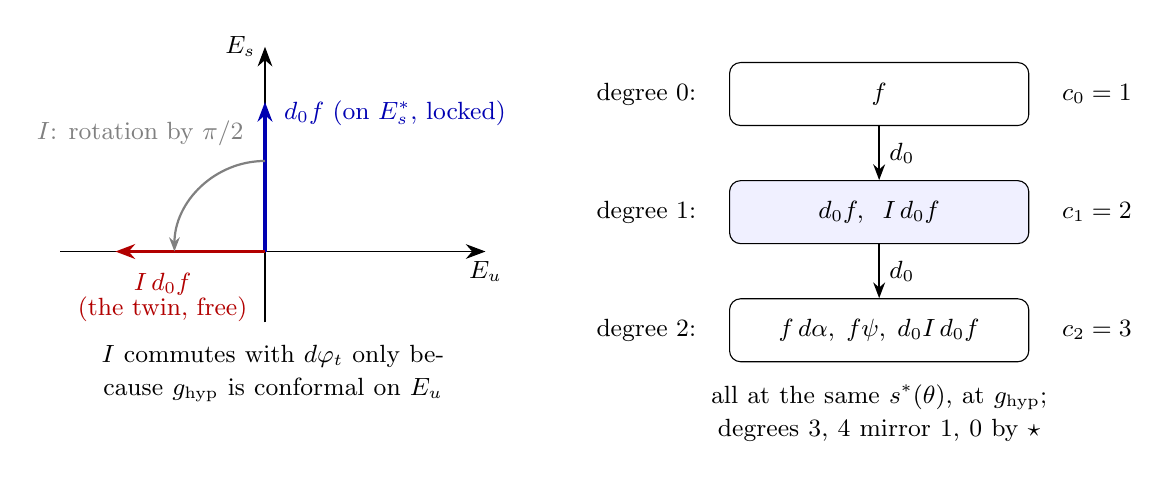
\begin{tikzpicture}[scale=1.0]
% left: E_u + E_s plane
\begin{scope}[xshift=0cm]
\draw[-{Stealth[length=2.5mm]}] (-2.6,0) -- (2.8,0) node[below] {\small $E_u$};
\draw[-{Stealth[length=2.5mm]}] (0,-0.9) -- (0,2.6) node[left] {\small $E_s$};
\draw[-{Stealth[length=2.5mm]}, very thick, blue!70!black] (0,0) -- (0,1.9);
\node[blue!70!black, anchor=west] at (0.12,1.75) {\small $d_0 f$ (on $E_s^*$, locked)};
\draw[-{Stealth[length=2.5mm]}, very thick, red!70!black] (0,0) -- (-1.9,0);
\node[red!70!black, align=center, anchor=north] at (-1.3,-0.15) {\small $I\,d_0 f$\\[-3pt]\small (the twin, free)};
\draw[-{Stealth[length=1.8mm]}, thick, gray] (0,1.15) arc (90:180:1.15);
\node[gray, anchor=east] at (-0.15,1.5) {\small $I$: rotation by $\pi/2$};
\node[align=center, text width=5.4cm] at (0.1,-1.55)
  {\small $I$ commutes with $d\varphi_t$ only because $g_{\mathrm{hyp}}$ is conformal on $E_u$};
\end{scope}
% right: degree ladder
\begin{scope}[xshift=7.8cm]
\node[draw, rounded corners, minimum width=3.8cm, minimum height=0.8cm] (d0) at (0,2.0) {\small $f$};
\node[draw, rounded corners, minimum width=3.8cm, minimum height=0.8cm, fill=blue!6] (d1) at (0,0.5) {\small $d_0 f,\;\; I\,d_0 f$};
\node[draw, rounded corners, minimum width=3.8cm, minimum height=0.8cm] (d2) at (0,-1.0) {\small $f\,d\alpha,\; f\psi,\; d_0 I\,d_0 f$};
\node[anchor=east] at (-2.2,2.0) {\small degree 0:};
\node[anchor=east] at (-2.2,0.5) {\small degree 1:};
\node[anchor=east] at (-2.2,-1.0) {\small degree 2:};
\draw[-{Stealth[length=2mm]}, thick] (d0) -- (d1) node[midway, right] {\small $d_0$};
\draw[-{Stealth[length=2mm]}, thick] (d1) -- (d2) node[midway, right] {\small $d_0$};
\node[anchor=west, align=left] at (2.2,2.0) {\small $c_0 = 1$};
\node[anchor=west, align=left] at (2.2,0.5) {\small $c_1 = 2$};
\node[anchor=west, align=left] at (2.2,-1.0) {\small $c_2 = 3$};
\node[align=center, text width=5.0cm] at (0,-2.05) {\small all at the same $s^*(\theta)$, at $g_{\mathrm{hyp}}$;\\ degrees 3, 4 mirror 1, 0 by $\star$};
\end{scope}
\end{tikzpicture}
\caption{The twin. Left: in the $E_u \oplus E_s$ plane the locked state $d_0 f$ and its rotation
$I\,d_0 f$ are independent resonant 1-forms at the same $s^*$. Right: the cluster at $s^*$ across
degrees, $c = (1,2,3,2,1)$, net order $1-2+3-2+1 = +1$: one simple zero of $\zeta$ at $s^*$, as
Fried's factorization at the hyperbolic metric requires ($\zeta(0; g_{\mathrm{hyp}}) = \tau_R$,
finite and nonzero). The partner $-s^*$ carries a second simple zero (state $f'\omega_s$). In the
Lean statement the degree-2 spectrum $\{s^*, s^*, s^*, -s^*\}$ at $\tau = 0$ is the hypothesis
\texttt{hmirror}.}
\end{figure}

\section{The second dial $\tau$: a conformal deformation unlocks the twin}

Now deform the metric conformally, $g_\tau = e^{-2\tau b} g_{\mathrm{hyp}}$, with $b$ in the
open dense set of functions for which CDDP's first variation is nondegenerate. (CDDP write the
deformation parameter as $s$; we write $\tau$ to keep $s$ for the spectral variable.) Pulling
the new geodesic flow back to the fixed phase space, the double point at $s^*$ splits. The two
velocities are read off CDDP's first-variation formula, equations (4.22) and (4.38): the locked
state moves with the degree-0 branch, at rate $O(\theta^2)$; the twin moves at rate
\[
r_0 \;=\; -\frac{\int (b\circ\pi)\,\alpha\wedge du_\psi\wedge du_\psi^*}{\langle\!\langle u_\psi,\, d\alpha\wedge u_\psi^*\rangle\!\rangle}
\;\neq\; 0 ,
\]
real, with $O(\theta^2)$ corrections. Write $s_{\mathrm{nc}}(\theta,\tau)$ for the twin's
position, so $s_{\mathrm{nc}}(\theta,0) = s^*(\theta) \approx -\mu_0/2$ and
$\partial_\tau s_{\mathrm{nc}}(0,0) = r_0$. In the Lean statement the first-variation formula
is the hypothesis \texttt{h422} (the pairing matrix $B$ and $B\cdot\partial_\tau M(0,0) =
\operatorname{diag}(0,p)$) and $r_0 = B_{cc}\,p/\det B > 0$ is \texttt{hr}$_0$; the twin is the
larger root $s^* + \tau\,w_+$ of the characteristic polynomial of $M$.

Two facts make the walk to zero unavoidable rather than accidental. \emph{Reality:} the twisted
resonance set is symmetric under $s \mapsto \bar s$ for every unitary $\rho$ (Hermitian adjoint
composed with time reversal $J(x,v) = (x,-v)$ preserves $\rho$; complex conjugation sends $\rho$
to $\bar\rho$ and, for the character family, $\theta$ to $-\theta$). A simple resonance near the
real axis is therefore real, and stays real along a real one-parameter family. \emph{No mirror:}
there is no $s \mapsto -\bar s$ symmetry off $g_{\mathrm{hyp}}$, so nothing stops a real
resonance from passing through $0$. Hence $\{g : 0 \in \operatorname{Res}\}$ is locally the zero
set of one real-analytic function: crossing has \textbf{codimension one}. The implicit function
theorem at $(\theta,\tau) = (0,0)$ gives the crossing curve
\[
\sigma(\theta) \;=\; \frac{\mu_0(\theta)}{2 r_0} + O(\theta^4)
\;=\; \frac{\theta^2\,\|\omega\|^2}{2 r_0 \operatorname{vol}(Z)} + O(\theta^4),
\qquad s_{\mathrm{nc}}(\theta, \sigma(\theta)) \equiv 0 .
\]
At $(g_{\sigma(\theta)}, \chi_\theta)$ the twin is a nonzero, non-closed, twisted resonant 1-form
at $s = 0$; the character is still acyclic (cohomology does not see the metric) and the metric is
still negatively curved with $|K+1| = O(\theta^2)$. The Lean statement proves existence and
uniqueness of the crossing in $(0, 2|s^*|/r_0]$ from \texttt{hdouble}, \texttt{h422},
\texttt{hr}$_0$ and the regularity of $M$; the parabola above is the informal sharpening.

\begin{figure}[h]
\centering
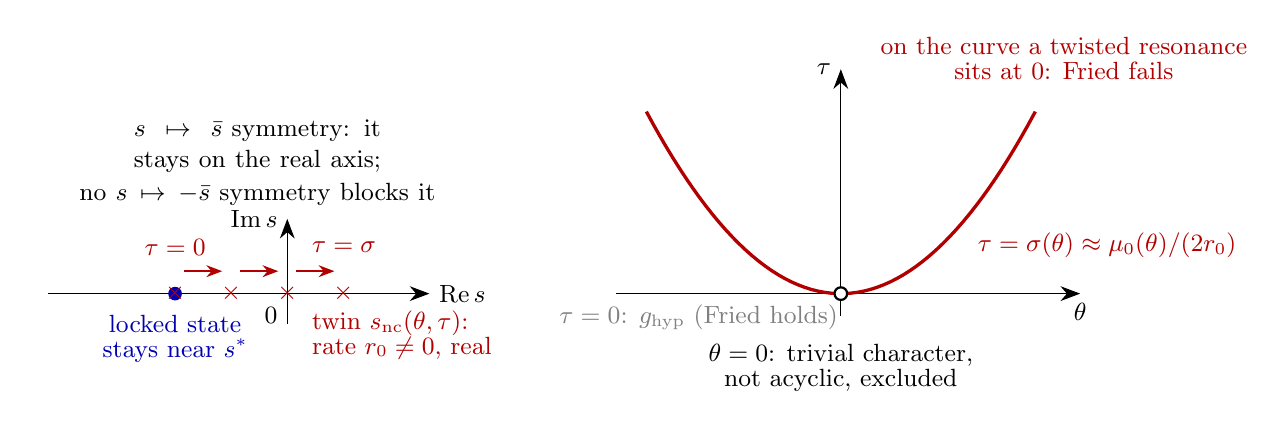
\begin{tikzpicture}[scale=0.95]
% left panel: s-plane, twin moving through 0
\begin{scope}[xshift=0cm]
\node[align=center, text width=5.6cm] at (-0.4,1.75) {\small $s \mapsto \bar s$ symmetry: it stays on the real axis;\\ no $s \mapsto -\bar s$ symmetry blocks it};
\draw[-{Stealth[length=2.5mm]}] (-3.2,0) -- (1.9,0) node[right] {\small $\operatorname{Re} s$};
\draw[-{Stealth[length=2.5mm]}] (0,-0.4) -- (0,1.0) node[left] {\small $\operatorname{Im} s$};
\node[below left] at (0,-0.05) {\small $0$};
% locked state stays at s* (the twin starts on top of it)
\fill[blue!70!black] (-1.5,0) circle (2.6pt);
\node[blue!70!black, align=center] at (-1.5,-0.6) {\small locked state\\[-3pt]\small stays near $s^*$};
% twin positions on the real axis, arrows just above
\foreach \x in {-1.5,-0.75,0,0.75} { \node[red!70!black] at (\x,0) {\small $\times$}; }
\draw[-{Stealth[length=2mm]}, thick, red!70!black] (-1.38,0.3) -- (-0.87,0.3);
\draw[-{Stealth[length=2mm]}, thick, red!70!black] (-0.63,0.3) -- (-0.12,0.3);
\draw[-{Stealth[length=2mm]}, thick, red!70!black] (0.12,0.3) -- (0.63,0.3);
\node[red!70!black] at (-1.5,0.62) {\small $\tau=0$};
\node[red!70!black, anchor=west] at (0.2,0.62) {\small $\tau=\sigma$};
\node[red!70!black, align=left, anchor=west] at (0.2,-0.55) {\small twin $s_{\mathrm{nc}}(\theta,\tau)$:\\[-3pt]\small rate $r_0 \neq 0$, real};
\end{scope}
% right panel: (theta, tau) parameter plane
\begin{scope}[xshift=7.4cm]
\draw[-{Stealth[length=2.5mm]}] (-3.0,0) -- (3.2,0) node[below] {\small $\theta$};
\draw[-{Stealth[length=2.5mm]}] (0,-0.3) -- (0,3.0) node[left] {\small $\tau$};
\node[gray] at (-1.9,-0.32) {\small $\tau = 0$: $g_{\mathrm{hyp}}$ (Fried holds)};
% crossing curve tau = c theta^2
\draw[very thick, red!70!black, domain=-2.6:2.6, samples=60] plot (\x, {0.36*\x*\x});
\node[red!70!black, anchor=west] at (1.7,0.65) {\small $\tau = \sigma(\theta) \approx \mu_0(\theta)/(2 r_0)$};
\node[red!70!black, align=center, anchor=west] at (0.4,3.15) {\small on the curve a twisted resonance\\[-3pt]\small sits at $0$: Fried fails};
% excluded origin
\draw[fill=white, thick] (0,0) circle (2.4pt);
\node[align=center, anchor=north] at (0,-0.55) {\small $\theta = 0$: trivial character,\\[-3pt]\small not acyclic, excluded};
\end{scope}
\end{tikzpicture}
\caption{The second dial. Left: as $\tau$ grows the twin walks along the real axis at rate $r_0$
and passes through $0$ at $\tau = \sigma(\theta)$; the locked state stays with the scalar
branch. Right: in the $(\theta,\tau)$ plane the crossing locus is a real-analytic curve through
the origin, tangent to the $\theta$-axis, even in $\theta$; drawn with $r_0 > 0$. The
$\theta$-axis is the hyperbolic metric. The origin itself is the trivial character and is
excluded. On the curve a twisted resonance sits at $0$; off it none does.}
\end{figure}

\section{Zero and pole arrive at different speeds}

What does the crossing do to $\zeta$? The exponent rule is
$\zeta = \prod_k Z_{X(k)}^{(-1)^k}$: degree-0, 2, 4 resonances are zeros, degree-1, 3 resonances
are poles. Follow the twin $u_{\mathrm{nc}}$ off the hyperbolic metric. It drags a chain with
it: $d_0 u_{\mathrm{nc}} \neq 0$ in degree 2 and $L u_{\mathrm{nc}} = d\alpha\wedge u_{\mathrm{nc}}$
in degree 3 are resonant at the same $s_{\mathrm{nc}}$, a $(0,1,1,1,0)$ cluster of net order
$-1+1-1 = -1$: \textbf{a pole of $\zeta$}, heading for $0$ at rate $r_0$. In the Lean statement
the lift $d_0 u_{\mathrm{nc}}$ is the hypothesis \texttt{hlocked}: every eigenvalue of $M$ is an
eigenvalue of $A$.

Meanwhile the degree-2 cluster has rank 4. Two of its branches are the locked branches (the
lifts of the closed branch and of the twin); the other two are the \emph{pure} degree-2
resonances $\beta_3, \beta_4$, the roots of $Q = X^2 - e_1 X + e_2$, each a simple zero of
$\zeta$. At $g_{\mathrm{hyp}}$ they sit at $\pm s^*$ (states $f\psi$ and $f'\omega_s$, the second
from the stable area form, which lands exactly at $-s^*$). At $\theta = 0$ they are pinned at
$0$ for every $\tau$ (CDDP Cor 4.1: $m_{2,0}(0) = b_1 + 2$, so the pole leaves $0$ \emph{alone};
in Lean, \texttt{hpinning}). Two consequences follow for their sum $e_1 = \beta_3+\beta_4$ and
product $e_2 = \beta_3\beta_4$. First, $e_1$ vanishes on both axes, so $e_1(\theta,\sigma(\theta))$
is small: $O(\theta^4)$ using evenness in $\theta$, and $|e_1(\theta,\sigma)| \le K_1|\theta|\sigma$
is what the Lean statement certifies from $C^2$ regularity alone. Second, at the crossing the
resonant complex must still be exact (Dang--Rivi\`ere; in Lean, \texttt{hexact}), and exactness
with $c_1 = c_3 = 1$, $c_0 = c_4 = 0$ forces $c_2 = 2c_1 = 2$: a pure degree-2 zero must arrive
at $0$ at the very instant the pole does, i.e.\ $e_2(\theta,\sigma)=0$. So the crossing cluster is
$c = (0,1,2,1,0)$, of order $-1+2-1 = 0$: \emph{$\zeta$ is regular and nonzero at $0$}. The pole
has been cancelled by a zero that is a \emph{different} resonance.

Cancelled, but not balanced. Near $\tau = \sigma$ the pole sits at $s_p \sim r_0(\tau-\sigma)$
and the arriving zero at $s_z = z(\theta,\tau)$, the pure branch nearest $0$, and
\[
\lim_{\tau\to\sigma}\frac{s_z}{s_p} \;=\; \frac{|s^*(\theta)|}{e_1(\theta,\sigma(\theta))}\,\big(1+O(\theta^2)\big)
\;=\; \frac{\Theta(\theta^2)}{O(\theta^4)} \;=\; \Theta(\theta^{-2}) \;\longrightarrow\; \infty .
\]
The zero comes in from farther and steeper: its slope at the crossing is $\Theta(\theta^{-2})\,r_0$,
against the pole's $r_0$. Lemma~A (the spectral-flow formula for the refined torsion of the
zero cluster: $(-1)^{Q_0}\tau(C^\bullet(0),\Gamma_\vartheta) = \lim\prod(-s_0(\tau))^{(-1)^q m(s_0(\tau))}$
over the resonances converging to $0$) then reads $\tau(C^\bullet(0)) = -\lim s_z/s_p$, and
Cauchy's formula on a fixed circle (Chaubet--Dang (6.5) read at $\lambda = 0$; in Lean,
\texttt{hfactor}) gives the value at the crossing:
\[
\zeta_{\chi_\theta}(0;\, g_{\sigma(\theta)}) \;=\; \tau_R \cdot \lim_{\tau\to\sigma}\frac{s_p}{s_z}
\;=\; \tau_R\cdot\frac{e_1(\theta,\sigma)}{|s^*(\theta)|} \;=\; \Theta(\theta^2)\,\tau_R \;\neq\; \tau_R .
\]
The Lean statement certifies the weaker, sufficient form: the twin's rate at the crossing is at
most $2r_0$, the zero's slope $\partial_\tau e_2/e_1$ exceeds $2r_0$ in modulus, so the ratio is
not $1$; the $\Theta(\theta^{\pm 2})$ sizes are the informal sharpening.

\begin{figure}[h]
\centering
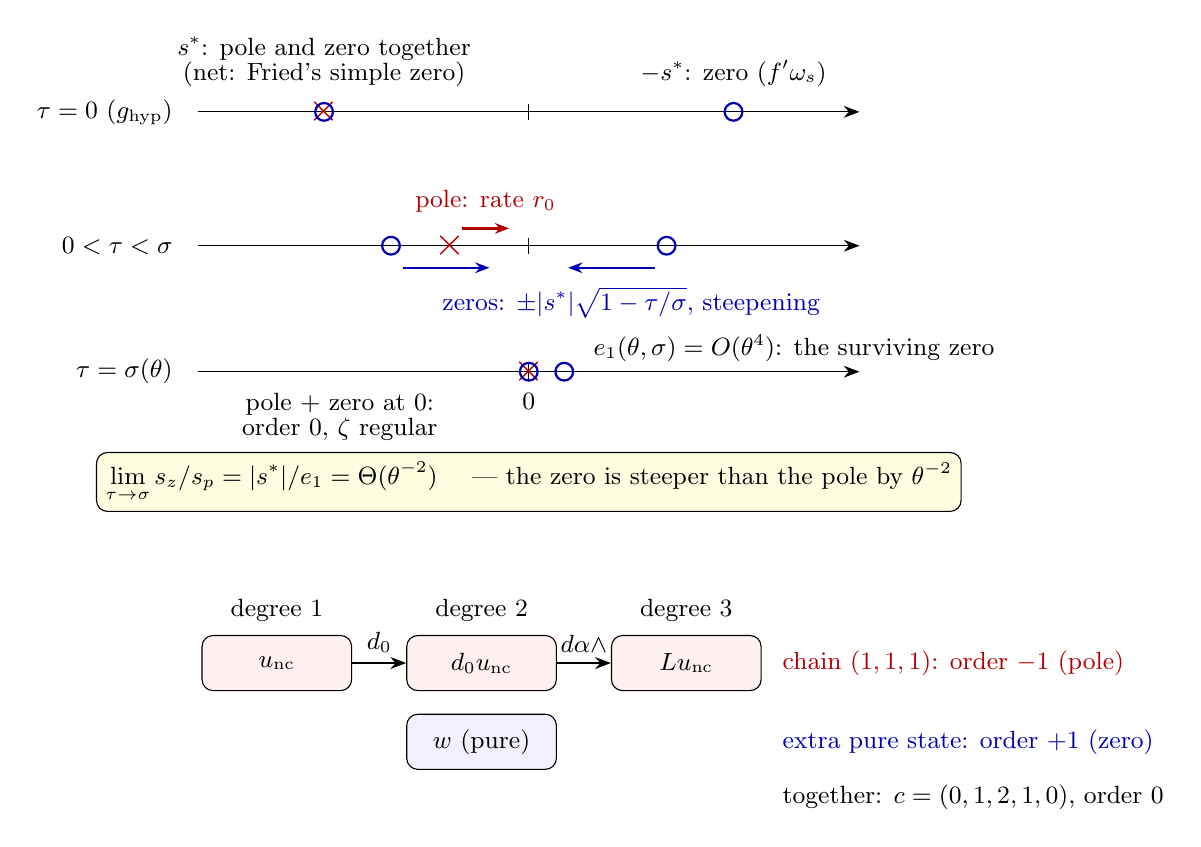
\begin{tikzpicture}[scale=1.0]
% three snapshots of the real s-axis near 0
\foreach \y/\lab in {4.2/{$\tau = 0$ ($g_{\mathrm{hyp}}$)}, 2.5/{$0 < \tau < \sigma$}, 0.9/{$\tau = \sigma(\theta)$}} {
  \draw[-{Stealth[length=2mm]}] (-4.2,\y) -- (4.2,\y);
  \draw (0,\y-0.1) -- (0,\y+0.1);
  \node[anchor=east] at (-4.4,\y) {\small \lab};
}
\node[below] at (0,0.75) {\small $0$};
% tau = 0: pole (x) and zero (o) coincide at s*, other zero at -s*
\node[red!70!black] at (-2.6,4.2) {\Large $\times$};
\draw[blue!70!black, thick] (-2.6,4.2) circle (3.2pt);
\draw[blue!70!black, thick] (2.6,4.2) circle (3.2pt);
\node[align=center, anchor=south] at (-2.6,4.4) {\small $s^*$: pole and zero together\\[-3pt]\small (net: Fried's simple zero)};
\node[anchor=south] at (2.6,4.4) {\small $-s^*$: zero ($f'\omega_s$)};
% 0 < tau < sigma: pole ahead, zeros at +-|s*|sqrt(1-tau/sigma)
\node[red!70!black] at (-1.0,2.5) {\Large $\times$};
\draw[blue!70!black, thick] (-1.75,2.5) circle (3.2pt);
\draw[blue!70!black, thick] (1.75,2.5) circle (3.2pt);
\draw[-{Stealth[length=1.8mm]}, thick, red!70!black] (-0.85,2.72) -- (-0.25,2.72);
\node[red!70!black, anchor=south] at (-0.55,2.8) {\small pole: rate $r_0$};
\draw[-{Stealth[length=1.8mm]}, thick, blue!70!black] (-1.6,2.22) -- (-0.5,2.22);
\draw[-{Stealth[length=1.8mm]}, thick, blue!70!black] (1.6,2.22) -- (0.5,2.22);
\node[blue!70!black, anchor=north] at (1.3,2.1) {\small zeros: $\pm|s^*|\sqrt{1-\tau/\sigma}$, steepening};
% tau = sigma: pole and one zero at 0, other zero at e1 = O(theta^4)
\node[red!70!black] at (0,0.9) {\Large $\times$};
\draw[blue!70!black, thick] (0,0.9) circle (3.2pt);
\draw[blue!70!black, thick] (0.45,0.9) circle (3.2pt);
\node[align=center, anchor=north] at (-2.4,0.75) {\small pole $+$ zero at $0$:\\[-3pt]\small order $0$, $\zeta$ regular};
\node[anchor=west] at (0.7,1.2) {\small $e_1(\theta,\sigma) = O(\theta^4)$: the surviving zero};
\node[draw, rounded corners, fill=yellow!12, align=center] at (0,-0.5)
  {\small $\displaystyle\lim_{\tau\to\sigma} s_z/s_p = |s^*|/e_1 = \Theta(\theta^{-2})$
   \quad --- the zero is steeper than the pole by $\theta^{-2}$};
% degree ladder below
\begin{scope}[yshift=-2.8cm]
\node[draw, rounded corners, minimum width=1.9cm, minimum height=0.7cm, fill=red!6] (a1) at (-3.2,0) {\small $u_{\mathrm{nc}}$};
\node[draw, rounded corners, minimum width=1.9cm, minimum height=0.7cm, fill=red!6] (a2) at (-0.6,0) {\small $d_0 u_{\mathrm{nc}}$};
\node[draw, rounded corners, minimum width=1.9cm, minimum height=0.7cm, fill=red!6] (a3) at (2.0,0) {\small $L u_{\mathrm{nc}}$};
\node[draw, rounded corners, minimum width=1.9cm, minimum height=0.7cm, fill=blue!6] (w) at (-0.6,-1.0) {\small $w$ (pure)};
\draw[-{Stealth[length=2mm]}, thick] (a1) -- (a2) node[midway, above] {\small $d_0$};
\draw[-{Stealth[length=2mm]}, thick] (a2) -- (a3) node[midway, above] {\small $d\alpha\wedge$};
\node[anchor=south] at (-3.2,0.4) {\small degree 1};
\node[anchor=south] at (-0.6,0.4) {\small degree 2};
\node[anchor=south] at (2.0,0.4) {\small degree 3};
\node[red!70!black, anchor=west] at (3.1,0) {\small chain $(1,1,1)$: order $-1$ (pole)};
\node[blue!70!black, anchor=west] at (3.1,-1.0) {\small extra pure state: order $+1$ (zero)};
\node[anchor=west] at (3.1,-1.7) {\small together: $c = (0,1,2,1,0)$, order $0$};
\end{scope}
\end{tikzpicture}
\caption{Different speeds. Top: three snapshots of the real axis near $0$. At $g_{\mathrm{hyp}}$
the pole ($\times$) and one pure zero ($\circ$) coincide at $s^*$ and net to Fried's simple zero;
as $\tau$ grows the pole moves at rate $r_0$ while the two pure zeros close in from $\pm|s^*|$
along a square root, steepening; at $\tau = \sigma$ the pole and one zero meet at $0$ and the
other zero rests at $e_1 = O(\theta^4)$. Bottom: the degree ladder at the crossing. The chain
through $d_0$ and $d\alpha\wedge$ is the pole; exactness forces one more pure degree-2 state, and
$c_2 = 2c_1$ makes the order zero. Regularity is exact; balance is not.}
\end{figure}

\section{The jump, and what survives}

Assemble the picture along the deformation. For $\tau \neq \sigma(\theta)$ no resonance is at
$0$, and DGRS Theorem~2 (local constancy of $\zeta(0)$ on the open set where $0$ is not a
resonance) together with Fried at $g_{\mathrm{hyp}}$ gives $\zeta_{\chi_\theta}(0; g_\tau) = \tau_R$
(in Lean, \texttt{hfried\_off}). At $\tau = \sigma(\theta)$ the value is $\Theta(\theta^2)\,\tau_R$.
So the function $g \mapsto \zeta_g(0)$ is constant on the hyperbolic component minus the crossing
hypersurface and takes a different value on it: a removable-looking discontinuity that is not
removable, because the value at the point is what Fried's identity is about. The factor
$\theta^2$ is an arrival ratio, not a property of the torsion: $\tau_R(\chi_\theta)$ is itself of
size $\theta^4$ at fixed $\theta$, and the jump is measured relative to it.

Chaubet--Dang's refinement reads the same picture without a jump. Their Theorem~4 says that
along any path of negatively curved metrics from $g_{\mathrm{hyp}}$,
$\zeta(s)^{(-1)^q} = |s|^{(-1)^q m}\,\tau_R\cdot\tau(C^\bullet(X_{g_0}))/\tau(C^\bullet(X_g))\,(1+O(s))$,
where $\tau(C^\bullet(X_g))$ is the refined torsion of the finite-dimensional zero-resonant
complex; Corollary~8 packages the leading Laurent coefficient times the cluster torsion into a
constant on connected open sets. On the crossing curve $m = 0$, the leading coefficient is
$\zeta(0) = \Theta(\theta^2)\tau_R$, and the cluster torsion is $|\tau(C^\bullet(0))| = |s^*|/e_1 = \Theta(\theta^{-2})$;
the product is $\tau_R$, continuous across the hypersurface. Off the curve the cluster is empty,
its torsion is $1$, and the two readings agree. The dynamical torsion is the invariant that does
not jump; the raw value $\zeta(0)$ is not. Readers who reserve the name ``Fried's conjecture''
for the resonance-free case will read the construction as an instance of the refined identity
rather than as a counterexample; the identity that fails is the naive one displayed in \S1.

\begin{figure}[h]
\centering
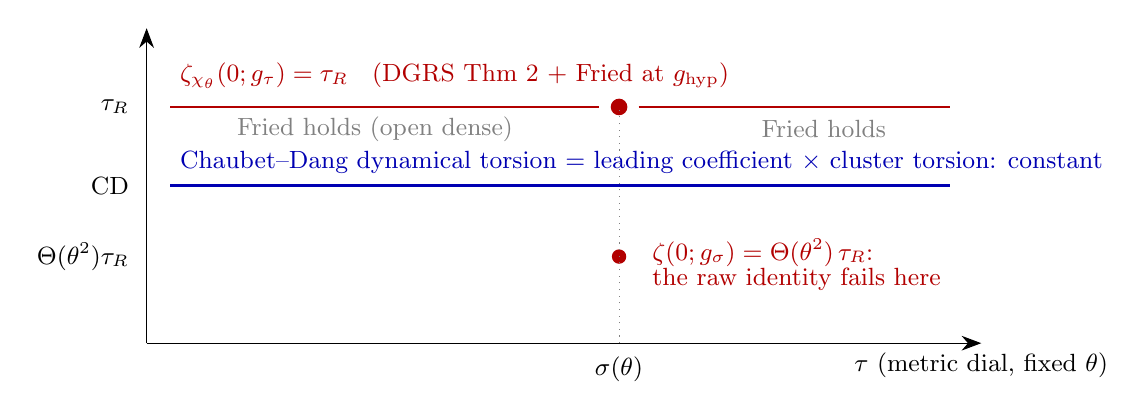
\begin{tikzpicture}[scale=1.0]
% axes
\draw[-{Stealth[length=2.5mm]}] (0,0) -- (10.6,0) node[below] {\small $\tau$ (metric dial, fixed $\theta$)};
\draw[-{Stealth[length=2.5mm]}] (0,0) -- (0,4.0);
% tau_R level
\draw[thick, red!70!black] (0.3,3.0) -- (5.75,3.0);
\draw[thick, red!70!black] (6.25,3.0) -- (10.2,3.0);
\draw[fill=white, thick, red!70!black] (6.0,3.0) circle (2.6pt);
\fill[red!70!black] (6.0,1.1) circle (2.6pt);
\draw[gray, dotted] (6.0,0) -- (6.0,3.0);
\node[below] at (6.0,-0.05) {\small $\sigma(\theta)$};
\node[red!70!black, anchor=west] at (0.3,3.4) {\small $\zeta_{\chi_\theta}(0; g_\tau) = \tau_R$ \; (DGRS Thm 2 $+$ Fried at $g_{\mathrm{hyp}}$)};
\node[red!70!black, anchor=west, align=left] at (6.3,1.0) {\small $\zeta(0; g_\sigma) = \Theta(\theta^2)\,\tau_R$:\\[-3pt]\small the raw identity fails here};
\node[anchor=east] at (-0.1,3.0) {\small $\tau_R$};
\node[anchor=east] at (-0.1,1.1) {\small $\Theta(\theta^2)\tau_R$};
% CD dynamical torsion: flat
\draw[very thick, blue!70!black] (0.3,2.0) -- (10.2,2.0);
\node[blue!70!black, anchor=west] at (0.3,2.3) {\small Chaubet--Dang dynamical torsion $=$ leading coefficient $\times$ cluster torsion: constant};
\node[anchor=east] at (-0.1,2.0) {\small CD};
% labels on the flat part
\node[gray] at (2.9,2.72) {\small Fried holds (open dense)};
\node[gray] at (8.6,2.72) {\small Fried holds};
\end{tikzpicture}
\caption{The jump. A one-dimensional slice of metric space at fixed $\theta \neq 0$. The raw
value $\zeta(0)$ (red) is flat at $\tau_R$ except at the single crossing point, where it drops
to $\Theta(\theta^2)\tau_R$: a value discontinuity with no order change. The dynamical torsion
(blue) is flat throughout, because the cluster torsion $\Theta(\theta^{-2})$ compensates exactly.
Fried at generic metrics of the hyperbolic component is a theorem (Humbert--Tao Thm~5 $+$ DGRS
Prop~7.7 $+$ Chaubet--Dang Thm~4); at the crossing metrics the raw identity fails and only the
refined one survives.}
\end{figure}

\noindent What survives, then, is the refined statement: the correct invariant at $s = 0$ is the
dynamical torsion, and Fried's conjecture as usually written needs the cluster factor at the
codimension-one set of metrics where a twisted resonance sits at $0$.

\section{Status}

\paragraph{What is machine-checked.} The Lean 4 / Mathlib theorem
\path{fried_counterexample_of_resolvent_inputs}, in the namespace \path{FriedCrossing}, is a
conditional reduction. Its statement of record is \path{Challenge.lean}, generated from the
statement-definitions module \path{B1s/fried_statement_defs_9_14.lean}; its proof is in
\path{B1s/fried_counterexample_main.lean} and the leg files that module imports. Its objects are two abstract resolvent families on Banach scales, complex structures
and nondegenerate frames, from which the cluster matrices $M$ and $A$ of \S1 are \emph{defined}
by contour integrals; its hypotheses are, in six groups, the properties of that data that the
argument uses, each cited to the literature: the two states at the double point
(\texttt{hstates}, \S4); the first variation and $r_0 > 0$ (\texttt{h422}, \texttt{hr}$_0$; CDDP
(4.22), (1.3)); the double point itself (\texttt{hdouble}; DGRS (7.6), Bunke--Olbrich, DFG); the
mirror spectrum at $\tau = 0$ (\texttt{hmirror}; DGRS (7.6)); the pinning at $\theta = 0$
(\texttt{hpinning}; CDDP Cor 4.1); the locked branches (\texttt{hlocked}; DGRS Lemma 7.1); and,
per $\theta$, the $\zeta$-side facts (\texttt{hfactor}, Chaubet--Dang (6.5); \texttt{hfried\_off},
DGRS Thm 2 with Fried at $g_{\mathrm{hyp}}$; \texttt{hexact}, Dang--Rivi\`ere; the dimension
bookkeeping \texttt{hacyc}, \texttt{hdual}, \texttt{hdims}). Its conclusion is that the twin
crosses $0$ at exactly one $\sigma \in (0, 2|s^*|/r_0]$, that $\zeta$ has order $0$ there, that
the zero's slope exceeds the pole's, and that
$\zeta(0; g_\sigma) = \tau_R\cdot(\text{pole rate})/(\text{zero rate}) \neq \tau_R$, with the
Lemma~A torsion identity. The theorem depends on no axiom beyond Lean's three standard ones, and
\texttt{leanprover/comparator} matches it constant by constant against the statement of record.

\paragraph{What is not.} The identification of the abstract data with the geometry --- that the
resolvent families are those of the twisted deformed generator on the anisotropic spaces of
$g_\tau$, that $\zeta_0(\tau)$ is the Ruelle zeta function of $g_\tau$ at $0$, that $\tau_R$ is
the Reidemeister torsion of $\chi_\theta$, and that the defined matrices are the cluster matrices
(their imaginary parts vanish) --- is the informal layer of this document and the accompanying
note. Nothing about manifolds, flows, anisotropic spaces or zeta functions is in Lean, and Lean
does not assert that data satisfying all the hypotheses at once exist. Of the hypotheses, only
the independence of $d_0 f$ and $I\,d_0 f$ inside \texttt{hstates} is derived (in \S4) rather
than read from a cited paper; the frame nondegeneracy is a choice. The $\Theta(\theta^{\pm 2})$
sizes drawn in \S6--\S7 are informal sharpenings of the certified inequalities.

\paragraph{Caveat.} This is a conditional reduction from cited inputs. It has not yet been
verified by a mathematician other than the author, and the claim that Fried's identity fails at
the crossing metric stands or falls with the six groups of cited facts holding as stated for the
geodesic flow.

\paragraph{Disclosure.} This document, the accompanying note and the Lean development were
produced with substantial assistance from Claude language models directed by the author, who
takes responsibility for the mathematics. The model roles are recorded in the repository's
metadata file \path{formalization.yaml}.

\end{document}
